\subsection{Runtime view}
An important issue in the project is the process in which the user gives a reply to an individual request
performed by a third party customer. This is exploited in the following diagram, that assumes that the user
has already logged in and that the list of pending request is non-empty.

\begin{figure}[H]
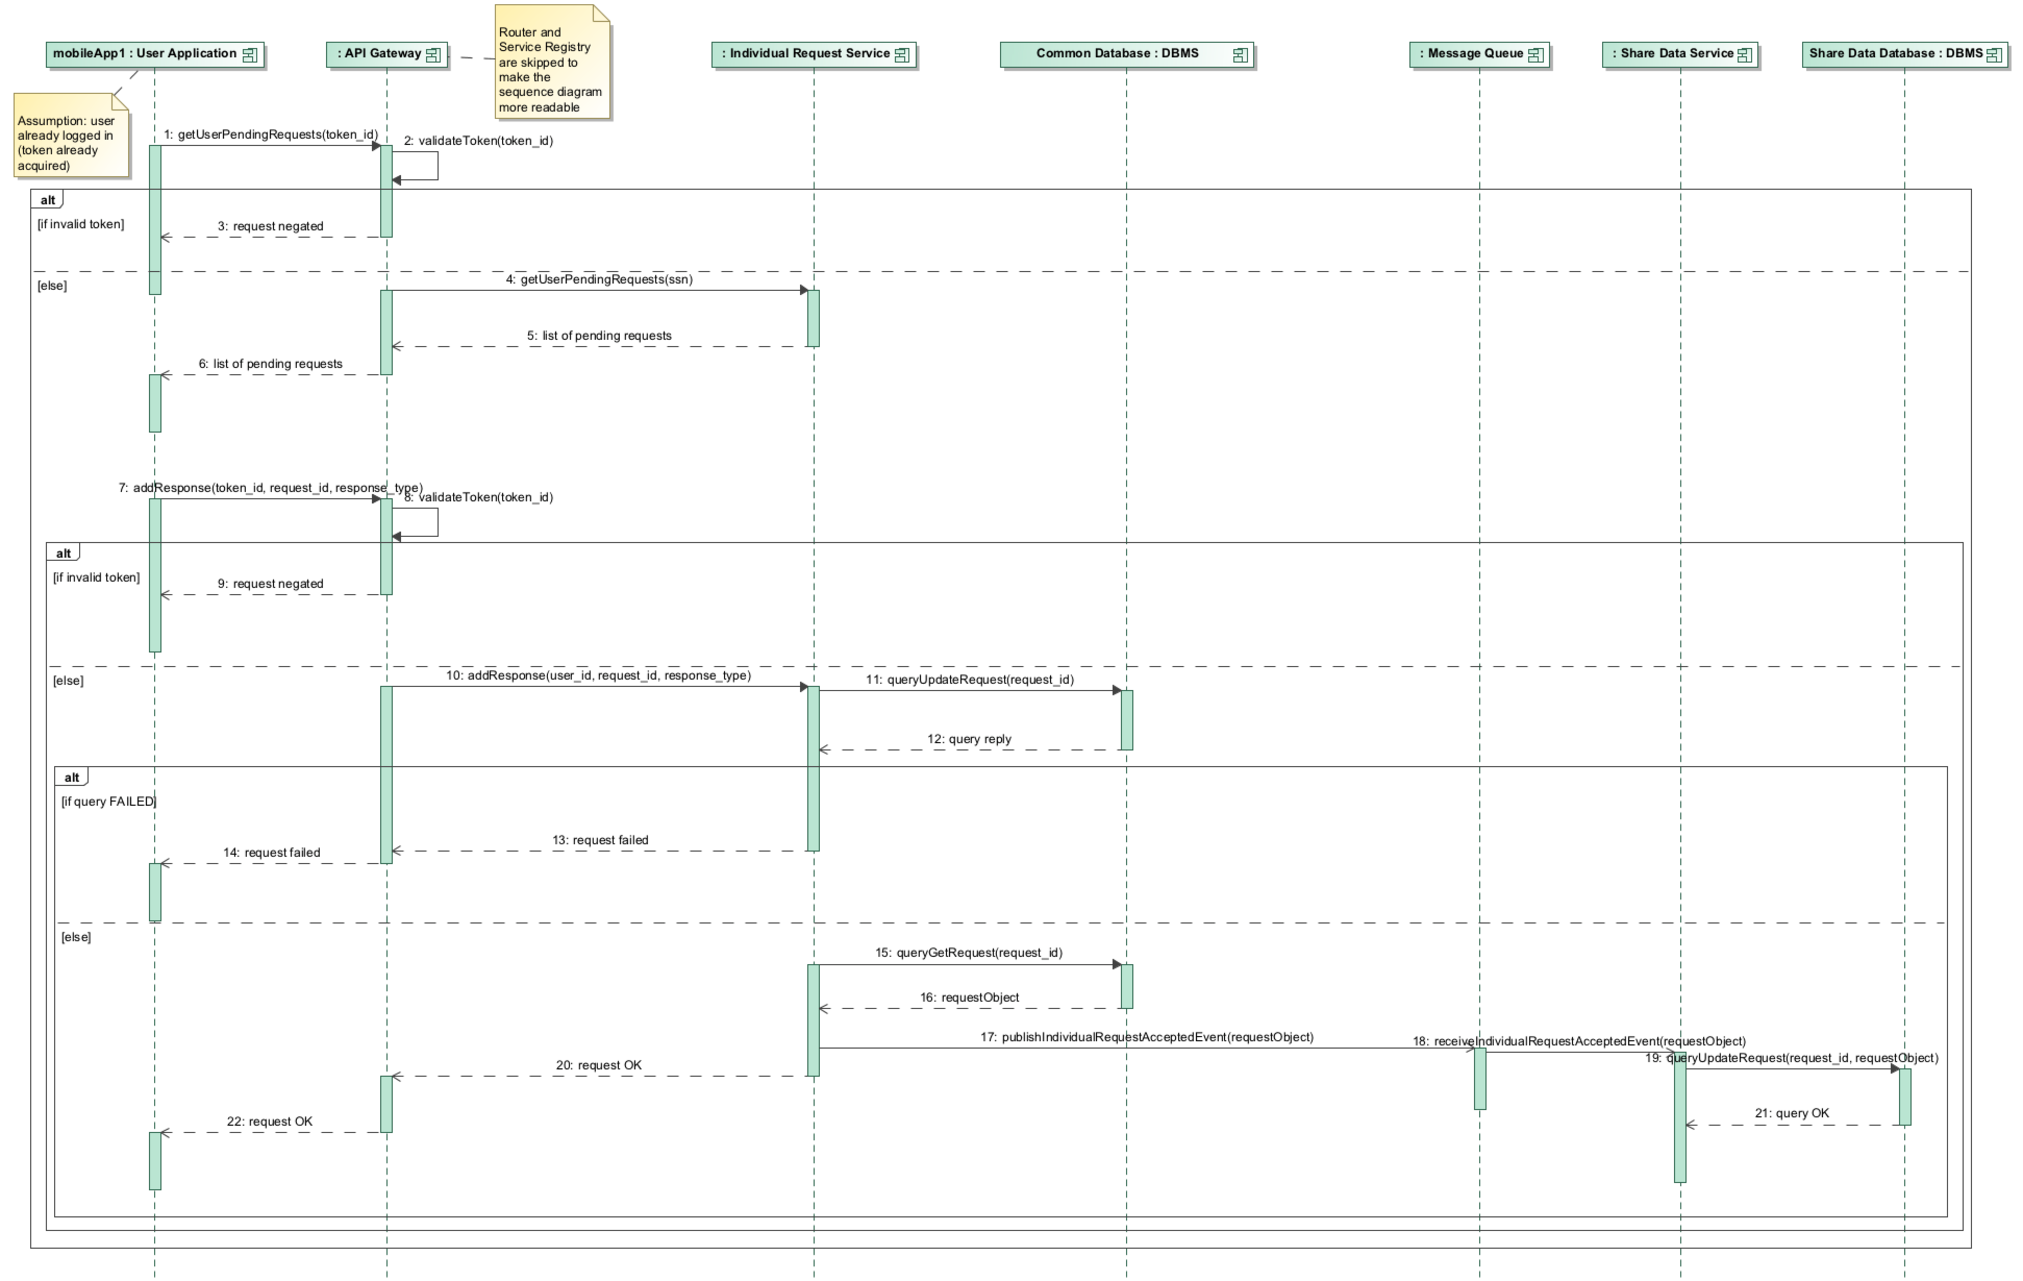
\includegraphics[width=\linewidth]{Images/requestacceptance.pdf}
\caption{ Sequence diagram: request acceptance }
\label{fig:world2}
\end{figure}

Some comments follows in order to clarify some essential points:
\begin{itemize}
\item The API gateway functions also as a proxy for the authentication service. In particular, he keeps track of the active sessions of the
users (identified by a token\_id). This information is in memory since
it was returned from the account service in the moment in which that user has performed the request
\item The communication between services is kept asynchronous, in order to not reduce the response time 
toward the user that initially used the individual request service. This is acceptable because there are
no strict requirement on the efficiency on the access of data by third party customer (i.e. the data should
not be available in the exact moment in which an user sends a response: some latency is tolerated). 
\item The share data needs information about requests that have been accepted, in order to correctly
provide the data access in the right way (i.e. granting access if an accepted request on the data has been 
accepted) 
\end{itemize}

\par 
Another important feature is the fact that third party customer can perform request on aggregated data.

\begin{figure}[H]
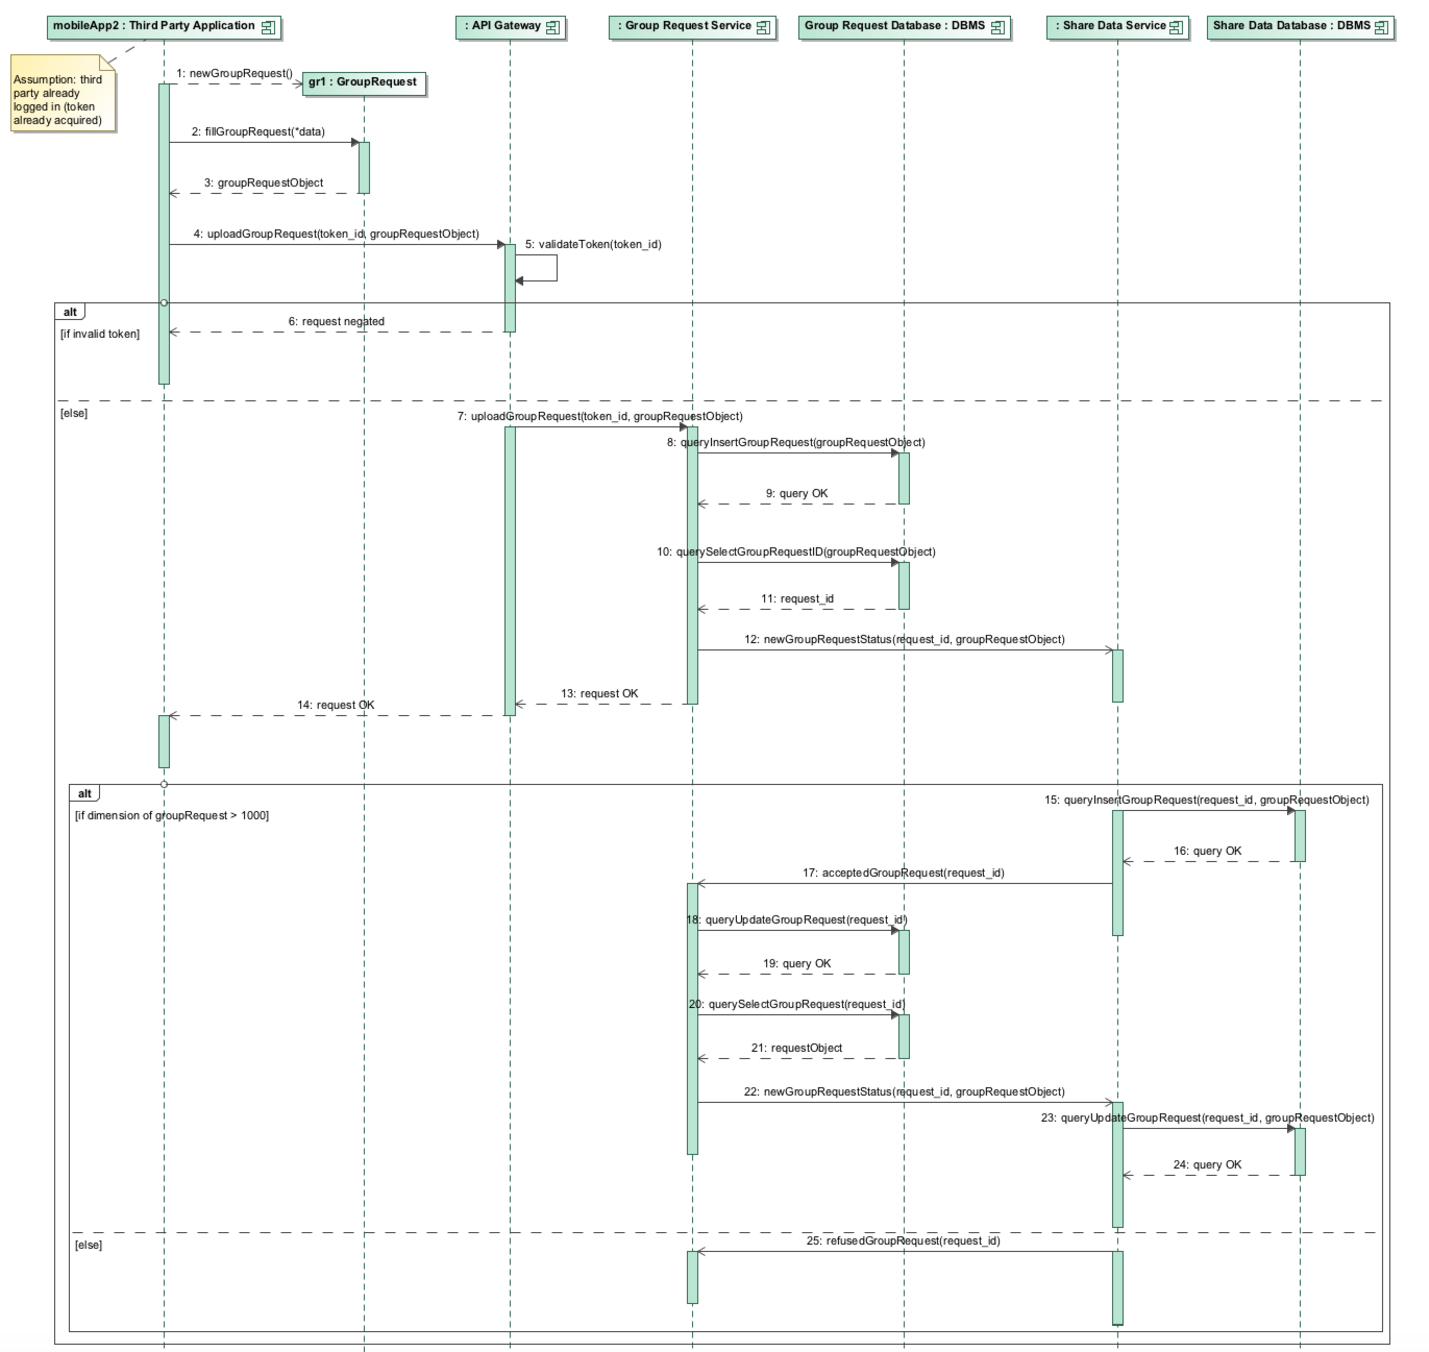
\includegraphics[width=\linewidth]{Images/grouprequest.pdf}
\caption{ Sequence diagram: group request }
\label{fig:world2}
\end{figure}

The same comments of the previous diagram hold, also, in this situation. 
However, it is relevant the fact 